% Copyright (c) 2009-2013 by the University of Waikato, Hamilton, NZ. 
% This work is made available under the terms of the 
% Creative Commons Attribution-ShareAlike 3.0 license, 
% http://creativecommons.org/licenses/by-sa/3.0/. 
%
% Version: $Revision: 3363 $

\documentclass[a4paper]{book}

\usepackage{wrapfig}
\usepackage{graphicx}
\usepackage{hyperref}
\usepackage{multirow}
\usepackage{scalefnt}
\usepackage{tikz}
\usepackage{varwidth}

% watermark -- for draft stage
\usepackage[firstpage]{draftwatermark}
\SetWatermarkLightness{0.9}
\SetWatermarkScale{5}

\hyphenation{ImageMagick}
\hyphenation{ImageJ}

% Copyright (c) 2009 by the University of Waikato, Hamilton, NZ. 
% This work is made available under the terms of the 
% Creative Commons Attribution-ShareAlike 3.0 license, 
% http://creativecommons.org/licenses/by-sa/3.0/. 
%
% Version: $Revision$

\newenvironment{tight_itemize}{
\begin{itemize}
  \setlength{\itemsep}{1pt}
  \setlength{\parskip}{0pt}
  \setlength{\parsep}{0pt}}{\end{itemize}
}

\newenvironment{tight_enumerate}{
\begin{enumerate}
  \setlength{\itemsep}{1pt}
  \setlength{\parskip}{0pt}
  \setlength{\parsep}{0pt}}{\end{enumerate}
}

% if you just need a simple heading
% Usage:
%   \heading{the text of the heading}
\newcommand{\heading}[1]{
  \vspace{0.3cm} \noindent \textbf{#1} \newline
}

\newcommand{\icon}[1]{\tikz[baseline=-3pt]\node[inner sep=0pt,outer sep=0pt]{\includegraphics[height=1.1em]{#1}};}


\title{
  \textbf{ADAMS} \\
  {\Large \textbf{A}dvanced \textbf{D}ata mining \textbf{A}nd \textbf{M}achine
  learning \textbf{S}ystem} \\
  {\Large Module: adams-imaging} \\
  \vspace{1cm}
  
\includegraphics[width=2cm]{images/imaging-module.png} \\
}
\author{
  Peter Reutemann
}

\setcounter{secnumdepth}{3}
\setcounter{tocdepth}{3}

\begin{document}

\begin{titlepage}
\maketitle

\thispagestyle{empty}
\center
\begin{table}[b]
	\begin{tabular}{c l l}
		\parbox[c][2cm]{2cm}{\copyright 2009-2013} &
		\parbox[c][2cm]{5cm}{
\includegraphics[width=5cm]{images/coat_of_arms.pdf}} \\
	\end{tabular}
	
\includegraphics[width=12cm]{images/cc.png} \\
\end{table}

\end{titlepage}

\tableofcontents
\listoffigures
%\listoftables


% %%%%%%%%%%%%%%%%%%%%%%%%%%%%%%%%%%
\chapter[Java Advanced
Imaging]{\parbox[b]{1.2cm}{
\includegraphics[width=1cm]{images/jai.png}}\parbox[c]{14cm}{Java
Advanced Imaging}}
Java Advanced Imaging (JAI) is an API to provide a simple, high-level
programming model which allows developers to create their own image manipulation
routines\footnote{\url{http://en.wikipedia.org/wiki/Java_Advanced_Imaging}{}}.

There are five JAI actors available:
\begin{tight_itemize}
    \item \texttt{source.JAICreateImage} -- for creating an empty image to be 
    forwarded.
	\item \texttt{transformer.JAIReader} -- for reading any image file that	JAI
	supports\footnote{\url{http://java.sun.com/products/java-media/jai/iio.html}{}} and forwarding a \texttt{BufferedImageContainer} object.
	\item \texttt{transformer.JAITransformer} -- performs a transformation
	using an existing JAI transformer class on the incoming image and
	outputs another image again.
	\item \texttt{transformer.JAIFlattener} -- turns a
	\texttt{BufferedImageContainer} into an \texttt{weka.core.Instance} object to
	be used in WEKA. The attaced meta-data in form of a report can be added to the
	output object as well.
	\item \texttt{sink.JAIWriter} -- for writing a \texttt{BufferedImageContainer}
	to a file format that JAI supports. If the image type cannot be
	determined based on the extension, you can also specify which type to generate.
\end{tight_itemize}

Figure \ref{jai-blur-flow} shows a
flow\footnote{adams-imaging-gaussian\_blur.flow} for reading images, blurring
them using a gaussian blur transformer and displaying them side-by-side. Figures
\ref{jai-blur-output-original} and \ref{jai-blur-output-blurred} show original
and blurred image.

\begin{figure}[htb]
  \centering
  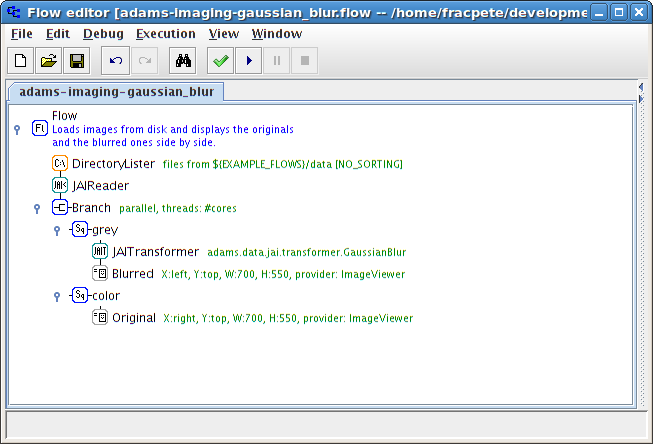
\includegraphics[width=10.0cm]{images/jai-blur-flow.png}
  \caption{JAI flow for blurring images stored in a directory.}
  \label{jai-blur-flow}
\end{figure}

\begin{figure}[htb]
  \begin{minipage}[b]{0.48\linewidth}
  \centering
  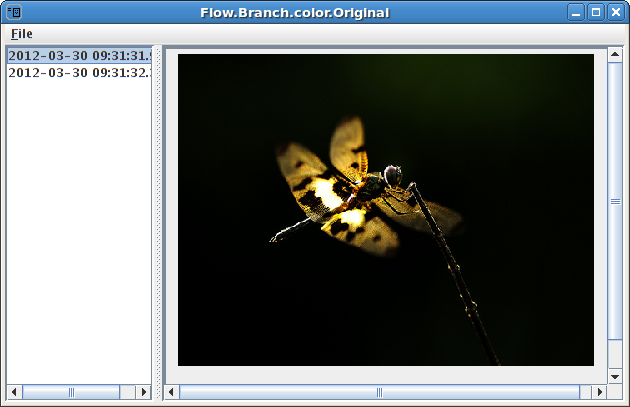
\includegraphics[height=3.7cm]{images/jai-blur-output-original.png}
  \caption{The original image.}
  \label{jai-blur-output-original}
  \end{minipage}%
  \begin{minipage}[b]{0.48\linewidth}
  \centering
  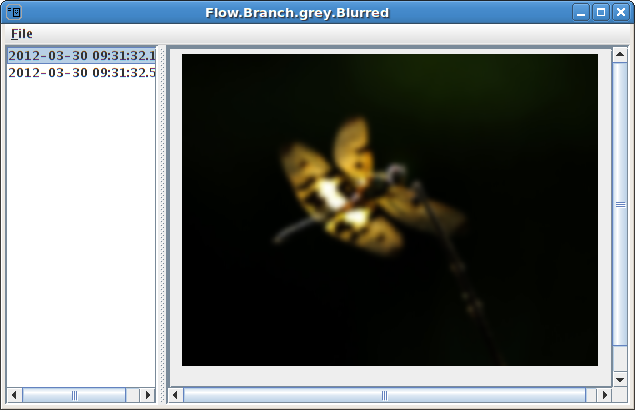
\includegraphics[height=3.7cm]{images/jai-blur-output-blurred.png}
  \caption{The blurred image.}
  \label{jai-blur-output-blurred}
  \end{minipage}
\end{figure}


%%%%%%%%%%%%%%%%%%%%%%%%%%%%%%%%%%%
\chapter[ImageJ]{\parbox[b]{1.2cm}{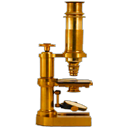
\includegraphics[width=1cm]{images/imagej.png}}\parbox[c]{14cm}{ImageJ}}
ImageJ is a public domain software suite written in Java (using AWT, opposed to
Swing which ADAMS uses) for image processing, developed at National Institutes 
of Health (\cite{imagej}).

\section{Flow}
There are four ImageJ actors available:
\begin{tight_itemize}
	\item \texttt{transformer.ImageJReader} -- for reading any image file that
	JAI supports\footnote{\url{http://imagejdocu.tudor.lu/doku.php?id=faq:general:which_file_formats_are_supported_by_imagej}{}}
	and forwarding an \texttt{ImagePlusContainer} object.
	\item \texttt{transformer.ImageJTransformer} -- performs a transformation
	using an existing ImageJ transformer class on the incoming image and
	outputs another image again. ImageJ plugin filters, commands and pre-recorded
	macros can be used to perform transformations.
	\item \texttt{transformer.ImageJFlattener} -- turns an
	\texttt{ImagePlusContainer} into an \texttt{weka.core.Instance} object to
	be used in WEKA. The attaced meta-data in form of a report can be added to the
	output object as well.
	\item \texttt{sink.ImageJWriter} -- for writing an \texttt{ImagePlusContainer}
	to a file format that ImageJ supports. If the image type cannot be
	determined based on the extension, you can also specify which type to generate.
\end{tight_itemize}

Figure \ref{imagej-greyscale-flow} shows a
flow\footnote{adams-imaging-transform\_to\_greyscale.flow} for reading images,
turning them into greyscale using a  transformer and displaying them
side-by-side.
Figures \ref{imagej-greyscale-output-original} and
\ref{imagej-greyscale-output-grey} show original and greyscale image.

\begin{figure}[htb]
  \centering
  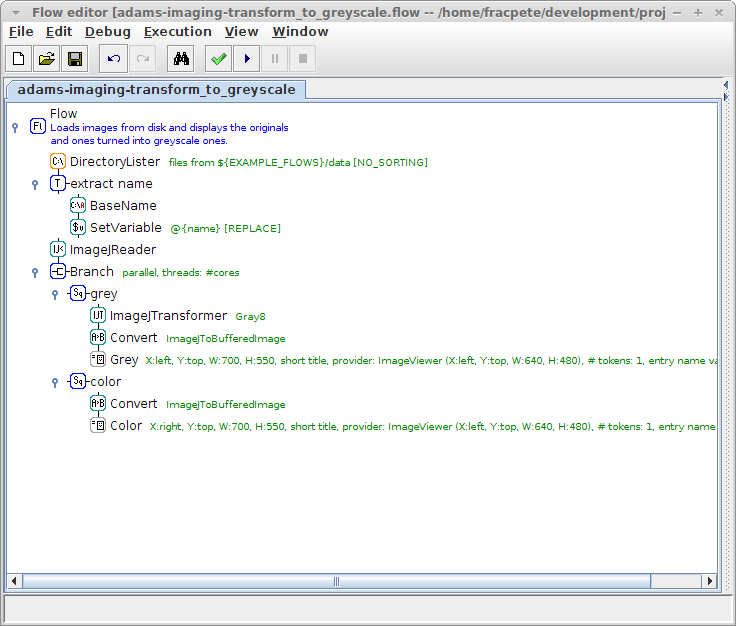
\includegraphics[width=10.0cm]{images/imagej-greyscale-flow.png}
  \caption{ImageJ flow for turning images stored in a directory into greyscale
  ones.}
  \label{imagej-greyscale-flow}
\end{figure}

\begin{figure}[htb]
  \begin{minipage}[b]{0.48\linewidth}
  \centering
  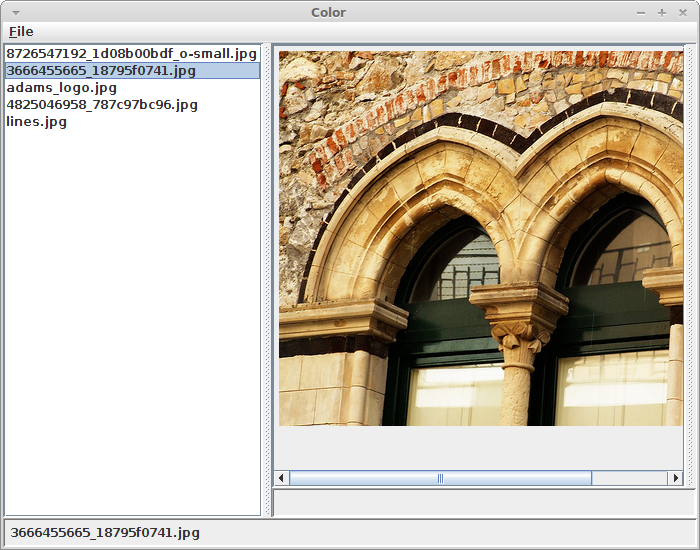
\includegraphics[height=3.7cm]{images/imagej-greyscale-output-original.png}
  \caption{The original image.}
  \label{imagej-greyscale-output-original}
  \end{minipage}%
  \begin{minipage}[b]{0.48\linewidth}
  \centering
  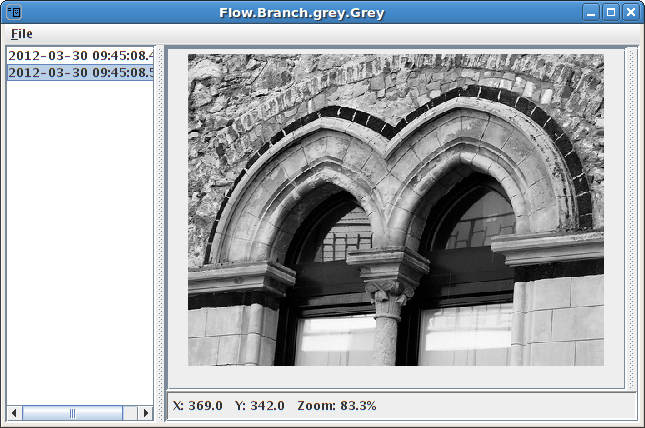
\includegraphics[height=3.7cm]{images/imagej-greyscale-output-grey.png}
  \caption{The greyscale image.}
  \label{imagej-greyscale-output-grey}
  \end{minipage}
\end{figure}

\clearpage
\section{Plugins}
By default, ADAMS includes plugins located in the following 
directory on Linux/Unix/Mac:
\begin{verbatim}
  $HOME/.adams/imagej/plugins
\end{verbatim}
and on Windows here:
\begin{verbatim}
  %USERPROFILE%/_adams/imagej/plugins
\end{verbatim}
You can override this directory by using the \texttt{ADAMS\_IMAGEJ\_DIR}
environment variable, which defines the directory one level above the 
\textit{plugins} directory. For instance, if your plugins directory is located
at:
\begin{verbatim}
  /home/user/imagej/plugins
\end{verbatim}
You have to define the \texttt{ADAMS\_IMAGEJ\_DIR} environment variable as 
follows:
\begin{verbatim}
  ADAMS_IMAGEJ_DIR=/home/user/imagej
\end{verbatim}


%%%%%%%%%%%%%%%%%%%%%%%%%%%%%%%%%%%
\chapter[ImageMagick]{\parbox[b]{1.2cm}{
\includegraphics[width=1cm]{images/imagemagick.png}}\parbox[c]{14cm}{ImageMagick}}
ImageMagick$\textsuperscript{\textregistered}$ is a software suite to create,
edit, compose, or convert bitmap images (\cite{imagemagick}). On Windows, in order to
process images with ImageMagick, you need to set the \texttt{IM4JAVA\_TOOLPATH} 
environment variable, pointing to the installation.

There are three ImageMagick actors available:
\begin{tight_itemize}
	\item \texttt{transformer.ImageMagickReader} -- for reading any image file that
	ImageMagick supports and forwarding a \texttt{BufferedImageContainer} object.
	\item \texttt{transformer.ImageMagickTransformer} -- performs any ImageMagick
	command on the incoming image that the \texttt{convert} tool\footnote{\url{http://www.imagemagick.org/script/convert.php}{}} supports and
	outputs another image again.
	\item \texttt{sink.ImageMagickWriter} -- for writing a \texttt{BufferedImageContainer}
	to a file format that ImageMagick supports. If the image type cannot be
	determined based on the extension, you can also specify which type to generate.
\end{tight_itemize}

There is no separate transformer for generating a WEKA instance, since the
ImageMagick actors process and output \texttt{BufferedImageContainer} objects as
well, just like the JAI actors. You can use the \texttt{JAIFlattener} for
generating WEKA output.

The example flow\footnote{adams-imaging-imagemagick\_script.flow} in Figure
\ref{imagemagick-resize-flow} loads a single photo from disk and then uses
ImageMagick to resize it to 90 by 90 pixels and scaling it by 200\% (see
\ref{imagemagick-resize-script}). Finally, the modified image is displayed in
the image viewer.

\begin{figure}[htb]
  \centering
  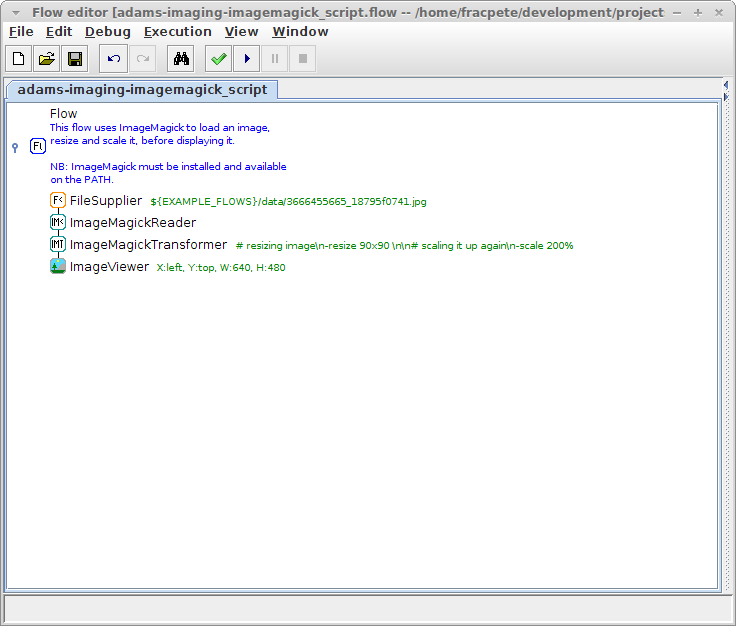
\includegraphics[width=10.0cm]{images/imagemagick-resize-flow.png}
  \caption{ImageMagick flow for processing (resizing) a single image.}
  \label{imagemagick-resize-flow}
\end{figure}

\begin{figure}[htb]
  \begin{center}
  \begin{varwidth}{\textwidth}
\begin{verbatim}
# resizing image
-resize 90x90
# scaling it up again
-scale 200%
\end{verbatim}
  \end{varwidth}
  \end{center}
  \caption{ImageMagick commands to resizing.}
  \label{imagemagick-resize-script}
\end{figure}

\begin{figure}[htb]
  \begin{minipage}[b]{0.48\linewidth}
  \centering
  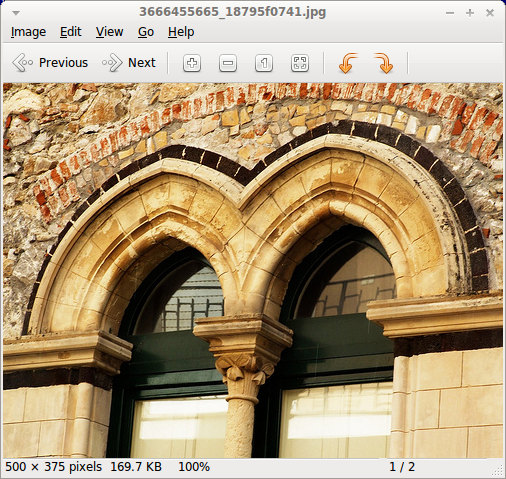
\includegraphics[height=3.8cm]{images/imagemagick-resize-original.png}
  \caption{The original image.}
  \label{imagemagick-resize-original}
  \end{minipage}%
  \begin{minipage}[b]{0.48\linewidth}
  \centering
  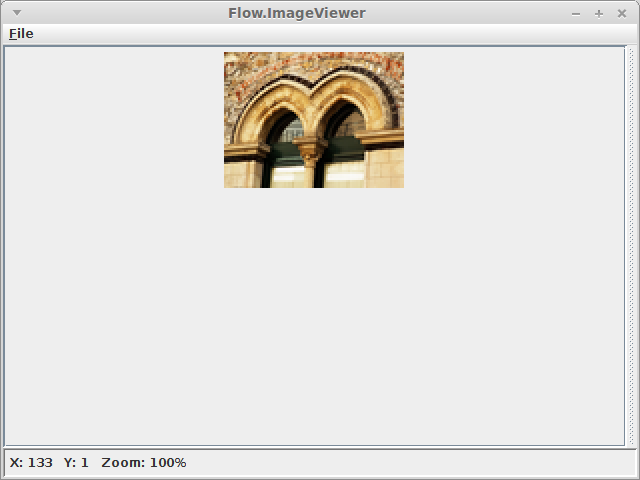
\includegraphics[height=3.8cm]{images/imagemagick-resize-output.png}
  \caption{The resized image.}
  \label{imagemagick-resize-output}
  \end{minipage}
\end{figure}

% %%%%%%%%%%%%%%%%%%%%%%%%%%%%%%%%%%
\chapter[BoofCV]{\parbox[b]{1.2cm}{
\includegraphics[width=1cm]{images/boofcv.png}}\parbox[c]{14cm}{BoofCV}}
BoofCV is an API for real-time computer vision and robotics applications\footnote{\url{http://boofcv.org/}{}}.

There are two BoofCV actors available:
\begin{tight_itemize}
	\item \texttt{transformer.BoofCVTransformer} -- performs a transformation
	using an existing BoofCV transformer class on the incoming image and
	outputs another image again.
	\item \texttt{transformer.BoofCVDetectLines} -- detects lines in images
	using a Hough line detector based on polar parametrization.
	\item \texttt{transformer.BoofCVFlattener} -- turns a
	\texttt{BoofCVImageContainer} into an \texttt{weka.core.Instance} object to
	be used in WEKA. The attaced meta-data in form of a report can be added to the
	output object as well.
\end{tight_itemize}


%%%%%%%%%%%%%%%%%%%%%%%%%%%%%%%%%%%
\chapter{Object conversion}
JAI and ImageMagick actors generate and accept a different type of token,
\textit{BufferedImageContainer} namely, which cannot be processed by ImageJ
actors. Vice versa, the tokens generated by ImageJ actors, of type
\textit{ImagePlusContainer}, are not accepted by JAI/ImagMagick actors. In order
to exchange data between the two domains, the \textit{Convert} transformer can
once again be used. 

The following conversions are available to convert from one
format into another:
\begin{tight_itemize}
	\item \textit{BoofCVImageToBufferedImage} -- for BoofCV to JAI/ImageMagick
	conversion.
	\item \textit{BufferedImageToBoofCV} -- for JAI/ImageMagick to BoofCV
	conversion.
	\item \textit{BufferedImageToImageJ} -- for JAI/ImageMagick to ImageJ
	conversion.
	\item \textit{ColorToHex} -- turns a Color object into its hexa-decimal 
	notation.
	\item \textit{ImageJToBufferedImage} -- converting from ImageJ to
	JAI/ImageMagick.
	\item \textit{HexToColor} -- turns a color in hexa-decimal notation back 
	into a Color object.
\end{tight_itemize}


%%%%%%%%%%%%%%%%%%%%%%%%%%%%%%%%%%%
\chapter{OCR}
A common task in image processing is \textit{optical character recognition} 
(OCR). ADAMS offers a simple wrapper around the open-source \textit{tesseract} 
engine \cite{tesseract}. The engine is available for Windows, Linux and Mac OSX.
It supports multiple languages, however, these need to be installed in order to
be actually available.

The follwoing actors are available:
\begin{tight_itemize}
	\item \textit{TesseractConfiguration} -- standalone for configuring OCR, 
	mainly to define where the tesseract executable is located.
	\item \textit{TesseractOCR} -- this transformer turns an image file into
	one or more text files, which need to be further processed in the flow
	then.\footnote{adams-imaging-ocr.flow}
\end{tight_itemize}

By default, the \textit{TesseractConfiguration} standalone uses the globally
defined preferences as default values. In the preferences dialog 
(\textit{Main menu $\rightarrow$ Program $\rightarrow$ Preferences 
$\rightarrow$ Tesseract}) you can specify the location of the tesseract
executable and the default language (see Figure \ref{tesseract-preferences}).
\begin{figure}[htb]
  \centering
  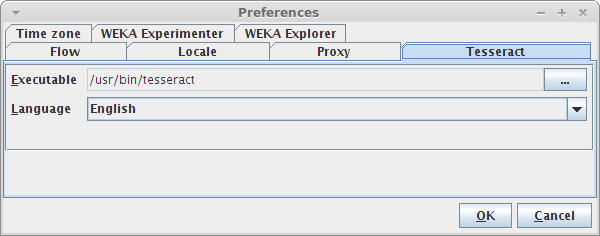
\includegraphics[width=10.0cm]{images/tesseract-preferences.png}
  \caption{Preferences for tesseract.}
  \label{tesseract-preferences}
\end{figure}


%%%%%%%%%%%%%%%%%%%%%%%%%%%%%%%%%%%
\chapter{Interaction}
The \textit{PixelSelector} transformer allows the user to interact with the
flow. The interaction with the user works as follows: an image viewer instance
is displayed when the \textit{PixelSelector} transformer receives an image token
as input. The use then right-clicks on a pixel that he wants to process, e.g.,
labelling for WEKA data generation. After all the pixels have been selected and
processed, the user then hits the \textit{OK} button to close the dialog. The
\textit{PixelSelector} then forwards the image container with the
attached, enriched report for further processing.

The \textit{PixelSelector} transformer is very generic, which means the actor
is responsible for the actions that the user can select from the right-click
menu. This is done by selecting the appropriate actions from the list of
available ones, e.g., \textit{AddClassification} (package
\texttt{adams.flow.transformer.pixelselector}), which is used for attaching
classification labels to pixels. In order to make these selections visible not
just in the report that is displayed on the right-hand side in the dialog,
appropriate overlays can be selected as well, e.g., the
\textit{ClassificationOverlay} (package
\texttt{adams.flow.transformer.pixelselector}) overlay, which displays the
pixels with the associated labels on the screen.

Figure \ref{pixelselector-flow} shows a
flow\footnote{adams-imaging-pixelselector.flow} that lets the user hand-label
all JPG images in a directory and generated WEKA data from it. It uses a cropped
region of 5x5 pixels around the selected pixels for the data generation. The
user interface for selecting the pixels is shown in Figure
\ref{pixelselector-interaction} and a resulting dataset in Figure
\ref{pixelselector-dataset}.

\begin{figure}[htb]
  \centering
  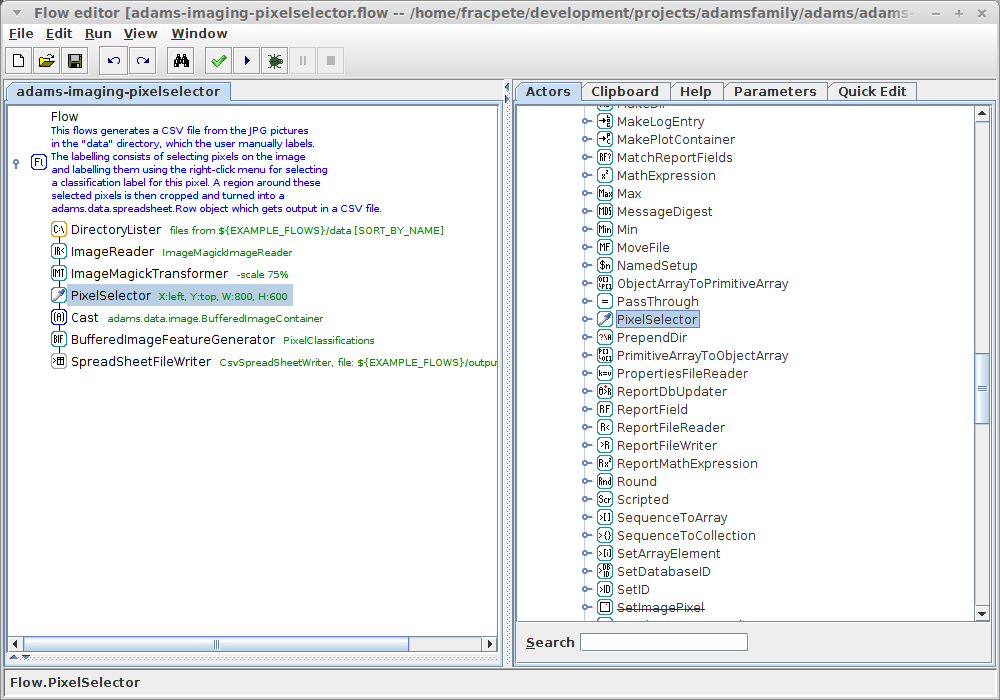
\includegraphics[width=10.0cm]{images/pixelselector-flow.png}
  \caption{Flow for generating ARFF file from user-labelled pixels.}
  \label{pixelselector-flow}
\end{figure}

\begin{figure}[htb]
  \centering
  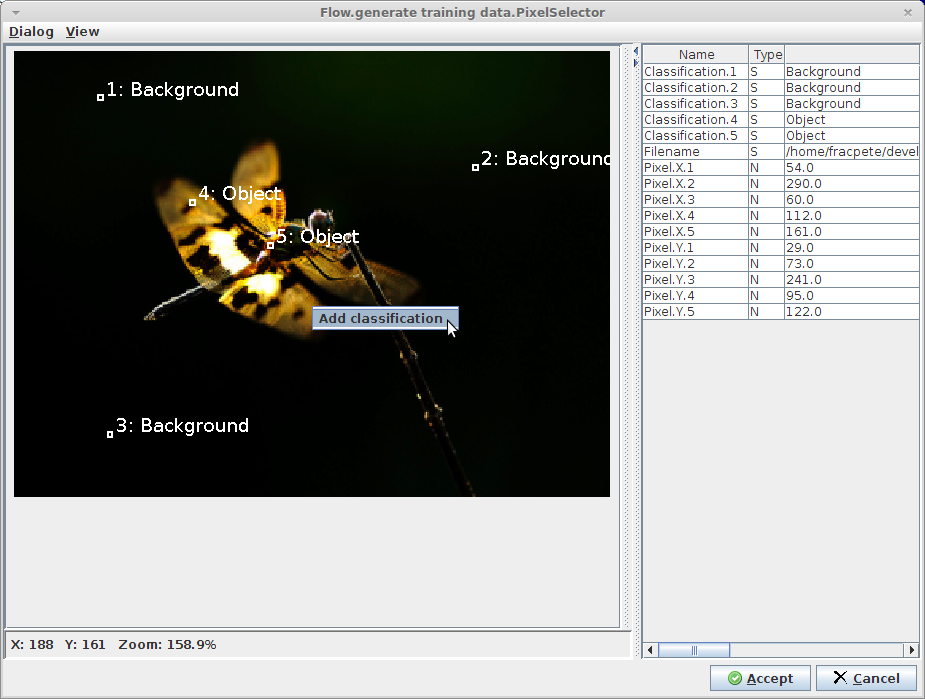
\includegraphics[width=10.0cm]{images/pixelselector-interaction.png}
  \caption{User interface for labelling pixels, displaying some pixels
  labelled already.}
  \label{pixelselector-interaction}
\end{figure}

\begin{figure}[htb]
  \centering
  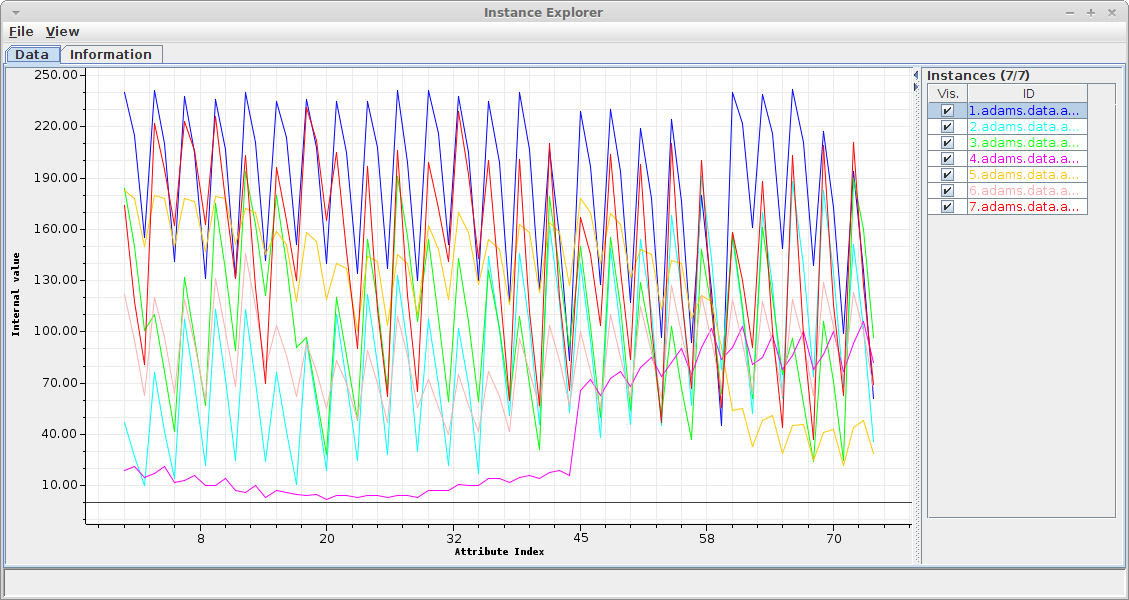
\includegraphics[width=10.0cm]{images/pixelselector-dataset.png}
  \caption{Example dataset generated using the PixelSelector.}
  \label{pixelselector-dataset}
\end{figure}

Of course, due to the interactive nature, labelling is performed on-the-fly and
no record is kept. Once the image has been processed, the
\textit{PixelSelector} will forget about it. If you want to preserve the
attached report, you can use the \textit{ReportFileWriter} transformer to save
the report to disk. 

In order to re-use a previously saved report, you can use the
\textit{SetReportFromFile} or \textit{SetReportFromSource} transformer to
replace the default report in the image container after you loaded the image
with the one stored on disk. This allows you to continue work with previously
generated labels, saving you a lot of work.

Since the \textit{SetReportFromFile} and \textit{SetReportFromSource}
transformers generate \textit{ReportHandler} tokens, you need to explicitly
cast the type of the tokens to the desired one, e.g.,
\textit{BufferedImageContainer}, using the \textit{Cast} control actor.

% %%%%%%%%%%%%%%%%%%%%%%%%%%%%%%%%%%
\chapter{WEKA output}
Of course, the data can be turned into a format that is suitable for WEKA
(\cite{weka}). For JAI and ImageMagick transformers, both generating
\textit{BufferedImageContainer} tokens, the \textit{JAIFlattener} can be used to
generate WEKA output in the form of \textit{weka.core.Instance} objects.
For ImageJ generated tokens, outputting \textit{ImagePlusContainer} tokens, you
have to use the \textit{ImageJFlattener} instead. This transformer also outputs
\textit{weka.core.Instance} objects. These \textit{Instance} objects can then be
processed further or simply dumped into a file. Figure
\ref{imagej-arff-generation-flow} shows a
flow\footnote{adams-imaging-arff\_generation.flow} that generates an ARFF file
from images using ImageJ. The resulting dataset, as displayed in the Instance
Explorer, is shown in Figure \ref{imagej-arff-generation-dataset}.

\begin{figure}[htb]
  \centering
  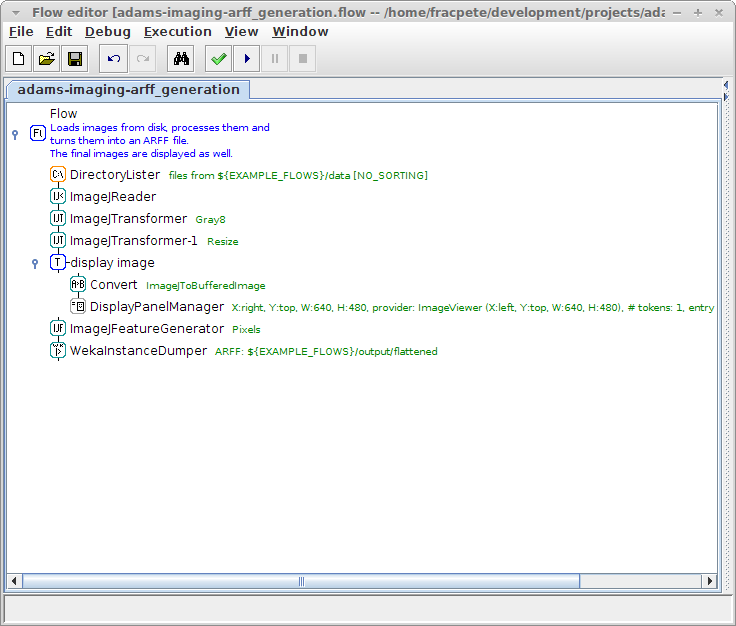
\includegraphics[width=10.0cm]{images/imagej-arff-generation-flow.png}
  \caption{Generating an ARFF file using ImageJ.}
  \label{imagej-arff-generation-flow}
\end{figure}

\begin{figure}[htb]
  \centering
  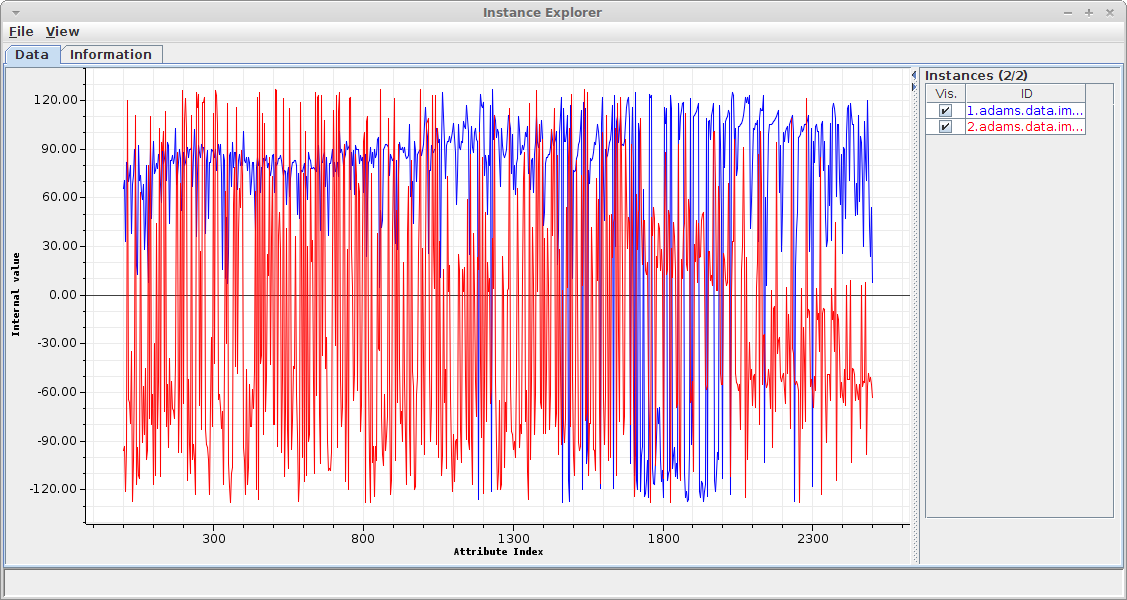
\includegraphics[width=10.0cm]{images/imagej-arff-generation-dataset.png}
  \caption{The ImageJ generated ARFF file.}
  \label{imagej-arff-generation-dataset}
\end{figure}


%%%%%%%%%%%%%%%%%%%%%%%%%%%%%%%%%%%
\chapter{Miscellaneous actors}
The imaging module offers some more actors that have not been introduced yet.

\noindent Available sources:
\begin{tight_itemize}
	\item \textit{ColorProvider} -- outputs Color objects generated by a 
	configured color provider.
\end{tight_itemize}

\noindent Available transformers:
\begin{tight_itemize}
	\item \textit{Draw} -- Performs draw operations on images, like setting 
	pixels, drawing lines, rectangles, ovals, text, images\footnote{adams-imaging-draw.flow}.
	\item \textit{ImageInfo} -- Allows you to obtain \textit{width} and
	\textit{height} information from an image.
	\item \textit{ImageMetaData} -- Extracts meta-data (EXIF or IPTC) from an
	image as spreadsheet.\footnote{adams-imaging-meta\_data.flow}
\end{tight_itemize}

\noindent Available sinks:
\begin{tight_itemize}
  \item \textit{FFmpeg} -- actor for processing videos using
  ffmpeg\cite{ffmpeg}\footnote{adams-imaging-ffmpeg.flow}.
\end{tight_itemize}


%%%%%%%%%%%%%%%%%%%%%%%%%%%%%%%%%%%
% Copyright (c) 2009-2012 by the University of Waikato, Hamilton, NZ. 
% This work is made available under the terms of the 
% Creative Commons Attribution-ShareAlike 4.0 license,
% http://creativecommons.org/licenses/by-sa/4.0/.
%
% Version: $Revision$

\begin{thebibliography}{999}
	% to make the bibliography appear in the TOC
	\addcontentsline{toc}{chapter}{Bibliography}

    % references
	\bibitem{adams}
		\textit{ADAMS} -- Advanced Data mining and Machine learning System \\
		\url{https://adams.cms.waikato.ac.nz/}{}

	\bibitem{esrigrid}
	 	\textit{Esri Grid} -- a raster GIS file format deveoped by Esri. \\
		\url{https://en.wikipedia.org/wiki/Esri\_grid}{}

	\bibitem{kml}
	 	\textit{Keyhole Markup Language} -- an XML notation for expressing
	 	geographic annotation and visualization within Internet-based,
	 	two-dimensional maps and three-dimensional Earth browsers. \\
		\url{http://en.wikipedia.org/wiki/Keyhole\_Markup\_Language}{}

	\bibitem{postgresql}
	 	\textit{PostgreSQL} -- a powerful, open source object-relational
	 	database system. \\
		\url{http://www.postgresql.org/}{}

	\bibitem{postgis}
		\textit{PostGIS} -- a spatial database extender for PostgreSQL
		object-relational database. It adds support for geographic
		objects allowing location queries to be run in SQL.  \\
		\url{http://postgis.net/}{}

	\bibitem{srid4269}
	 	\textit{SRID 4269} -- or NAD 83 (North American Datum). \\
		\url{http://spatialreference.org/ref/epsg/4269/}{}

	\bibitem{mysql}
		\textit{MySQL} -- an open-source relational database management
		system (RDBMS) \\
		\url{http://www.mysql.com/}{}

\end{thebibliography}


\end{document}
